\documentclass[11pt, a4paper]{article}

% Preamble: Packages and Document Setup
\usepackage[margin=1in]{geometry}
\usepackage{amsmath}
\usepackage{graphicx}
\usepackage{booktabs}
\usepackage{hyperref}
\usepackage{xcolor}
\usepackage{listings}
\usepackage{times}
\usepackage{float}

% Hyperlink setup
\hypersetup{
    colorlinks=true,
    linkcolor=blue,
    filecolor=magenta,      
    urlcolor=cyan,
}

% MATLAB code listing style
\definecolor{codegreen}{rgb}{0,0.6,0}
\definecolor{codegray}{rgb}{0.5,0.5,0.5}
\definecolor{codepurple}{rgb}{0.58,0,0.82}
\definecolor{backcolour}{rgb}{0.95,0.95,0.92}

\lstdefinestyle{matlabstyle}{
    backgroundcolor=\color{backcolour},   
    commentstyle=\color{codegreen},
    keywordstyle=\color{magenta},
    numberstyle=\tiny\color{codegray},
    stringstyle=\color{codepurple},
    basicstyle=\footnotesize\ttfamily,
    breakatwhitespace=false,         
    breaklines=true,                 
    captionpos=b,                    
    keepspaces=true,                 
    numbers=left,                    
    numbersep=5pt,                  
    showspaces=false,                
    showstringspaces=false,
    showtabs=false,                  
    tabsize=2,
    language=Matlab
}
\lstset{style=matlabstyle}

% Document Information
\title{\textbf{Project Report: A Numerical Investigation into the Unification of Antenna Theories}}
\author{Gemini \& Collaborator}
\date{\today}

\begin{document}

\maketitle
\hrule
\vspace{1em}

% --- Executive Summary ---
\section*{Executive Summary}
\addcontentsline{toc}{section}{Executive Summary}

This report details the development and application of a sophisticated computational tool in MATLAB to investigate the theoretical connections between the \textbf{Theory of Characteristic Modes (TCM)}, \textbf{Degrees of Freedom (DoF)}, and \textbf{Fundamental Radiative Limits} for a thin-wire dipole antenna. The project progressed through three distinct phases: initial tool development, an intensive collaborative debugging and enhancement cycle, and a final numerical experiment.

The core of the project was the creation of \texttt{main\_CMA\_Dipole.m}, a solver based on the Method of Moments (MoM). This tool underwent significant refinement to correct subtle but critical bugs in its physics engine, evolving into a production-ready, scientifically validated piece of software. The understanding that scientific software development is an iterative process was key; each iteration brought the simulation closer to physically accurate results.

The final numerical experiment involved sweeping the electrical length of a dipole antenna and analyzing its behavior from two distinct viewpoints: an "internal" perspective based on the characteristic mode eigenvalues and an "external" perspective based on the complexity of the far-field radiation.

The key findings are twofold:
\begin{enumerate}
    \item The analysis successfully validated the long-held theory that an electrically small antenna's effective radiating size is significantly larger than its physical size. This phenomenon is a direct consequence of the reactive energy stored around the antenna and has important implications for the design of compact antennas in modern devices.
    \item The investigation revealed that a simple eigenvalue-based criterion for counting "significant" modes is insufficient to fully describe the antenna's true Degrees of Freedom. The complexity of the external radiated field was found to be a more comprehensive and accurate metric. This finding refines our understanding of how internal modes relate to external antenna behavior.
\end{enumerate}
This work not only provides numerical evidence supporting established theories but also offers nuanced insights into their limitations, culminating in a robust and extensible solver for future antenna analysis.

\newpage

% --- Phase 1 ---
\section{Phase 1: Initial Tool Development}

The project began with the development of a foundational MATLAB script, \texttt{main\_CMA\_Dipole.m}. The objective was to create a solver capable of performing a Characteristic Mode Analysis (CMA) on a thin-wire dipole antenna. This choice was made due to the relative simplicity yet rich physics of the dipole as a fundamental radiating structure.

The core functionality of this initial version followed a clear algorithmic flow, which can be summarized in pseudocode:

\begin{lstlisting}[language=Matlab, caption={Pseudocode for the initial CMA solver logic.}, label={lst:pseudo1}]
function cma_solver(frequency, length, radius, segments)
  // 1. Geometry & MoM Assembly
  [z_center, dL] = create_dipole_geometry(length, segments);
  Z_matrix = calculate_impedance_matrix(z_center, dL, ...);

  // 2. Matrix Decomposition
  R = real( (Z_matrix + Z_matrix.')/2 );
  X = imag( (Z_matrix + Z_matrix.')/2 );

  // 3. Eigenproblem Solution
  [J_n, lambda_n] = eig(X, R);

  // 4. Basic Visualization
  plot_eigenvalues(lambda_n);
  plot_currents(J_n);
  plot_patterns(J_n);
end
\end{lstlisting}

Initial parameters, such as the number of segments ($N=41$), were chosen based on common practices in computational electromagnetics to provide a good balance between numerical accuracy and computational cost for the frequency range of interest. This initial script served as the engine for the entire project, but as a first draft, it contained latent bugs that would be uncovered in the next phase.

% --- Phase 2 ---
\section{Phase 2: Collaborative Refinement and Debugging}

This phase was the most critical and intensive part of the project. Through an iterative, collaborative process of testing, analysis, and refinement, the initial solver was transformed from a prototype into a scientifically accurate and robust tool. The development process was tracked using version numbers (e.g., v2.5, v8.0, v16.0) to ensure changes were documented and reproducible.

The key challenges and solutions during this phase were:
\begin{enumerate}
    \item \textbf{Memory Management:} The initial attempt to run a simulation sweep resulted in a memory overflow. This was resolved by adding a \texttt{close(gcf)} command after saving each figure, a crucial fix for enabling large-scale batch processing.
    \item \textbf{The Physics Engine Bug:} The most significant challenge was a deep bug in the mathematical "kernel" used to calculate the impedance matrix. The symptoms included zero directivity and non-physical eigenvalues. The debugging effort traced these symptoms back to their source: an incorrect formulation of the \textbf{Pocklington integral equation}. The correction of this formula represented a critical turning point.
    \item \textbf{Scientific and Usability Enhancements:} As the solver's accuracy improved, professional features were added:
    \begin{itemize}
        \item \textbf{New Scientific Metrics:} Calculations for Modal Quality Factor ($Q_n$) and Modal Significance ($MS_n$) were added.
        \item \textbf{Robustness:} Hard \texttt{assert} statements were replaced with forgiving warnings, and the code was made to gracefully handle cases where the parallel computing toolbox was unavailable.
        \item \textbf{User-Friendliness:} A summary table of key results is now printed to the command window.
    \end{itemize}
    \item \textbf{Programmatic Validation:} A companion script, \texttt{demo\_and\_validate\_CMA\_Solver.m}, was developed to serve as a unit test. This script runs a standard benchmark case and uses programmatic assertions to verify the physical accuracy of the results, ensuring that future code changes do not introduce regressions. The core of this validation is captured in these key lines:
\end{enumerate}

\begin{lstlisting}[language=Matlab, caption={Key assertion statements in the validation script, with explanatory comments.}, label={lst:assert}]
% Ensure the first eigenvalue is near zero, as expected for a resonant dipole.
assert(abs(lambda1_sim - target_lambda1) < tolerance_lambda1, ...
    'Validation Failed: Eigenvalue is outside the acceptable tolerance.');
   
% Ensure the directivity of the first mode is within 5% of the theoretical value.
assert(abs(D1_sim - target_D1)/target_D1 * 100 < tolerance_D1_percent, ...
    'Validation Failed: Directivity is outside the acceptable tolerance.');
\end{lstlisting}

By the end of this phase, \texttt{main\_CMA\_Dipole.m} had evolved into a production-ready solver, validated against known benchmarks and engineered for reliable, flexible use.

% --- Phase 3 ---
\section{Phase 3: Numerical Experiment \& Unification Analysis}

With a validated tool in hand, the final phase focused on executing the planned numerical experiment. The \texttt{run\_phase3\_unification\_analysis.m} script was created to automate the entire workflow.
\begin{enumerate}
    \item \textbf{Data Generation:} It called the \texttt{main\_CMA\_Dipole} solver in a loop over a range of electrical lengths ($L/\lambda$ from 0.1 to 1.5), running the simulation in a "silent" mode to collect the full data for each case. The results of each simulation were stored in a structured cell array in memory for subsequent analysis, avoiding the need for intermediate file I/O.
    \item \textbf{Dual-Perspective Analysis:} For each data point, the Degrees of Freedom (NDoF) were calculated. The far-field analysis relied on a helper function, \texttt{fit\_spherical\_waves.m}, which performs a least-squares fit of the radiated field to a basis of spherical wave functions. A standard 5\% error threshold was used to determine the minimum number of modes ($N_{min}$) required for an accurate representation, as shown in Listing \ref{lst:fit_call}.
    \item \textbf{Visualization:} It synthesized the analyzed data into the two "Grand Unification" plots.
\end{enumerate}

\begin{lstlisting}[language=Matlab, caption={Example call to the spherical wave fitting function within the analysis loop.}, label={lst:fit_call}]
% Set parameters for the spherical wave decomposition
max_N_to_test = 20;
fit_error_threshold = 0.05; % 5% error

% Find the minimum number of modes (N) needed to describe the pattern
N_Yaghjian(i) = fit_spherical_waves(theta, E_pattern, max_N_to_test, fit_error_threshold);
\end{lstlisting}

% --- Results ---
\section{Results and Scientific Interpretation}

The experiment produced two key figures that provide the central conclusions of this report.

\subsection{Figure 1: Unification of Degrees of Freedom}
This plot compares the NDoF calculated from the internal modes (TCM) against the NDoF calculated from the external field complexity.

\begin{figure}[H]
    \centering
    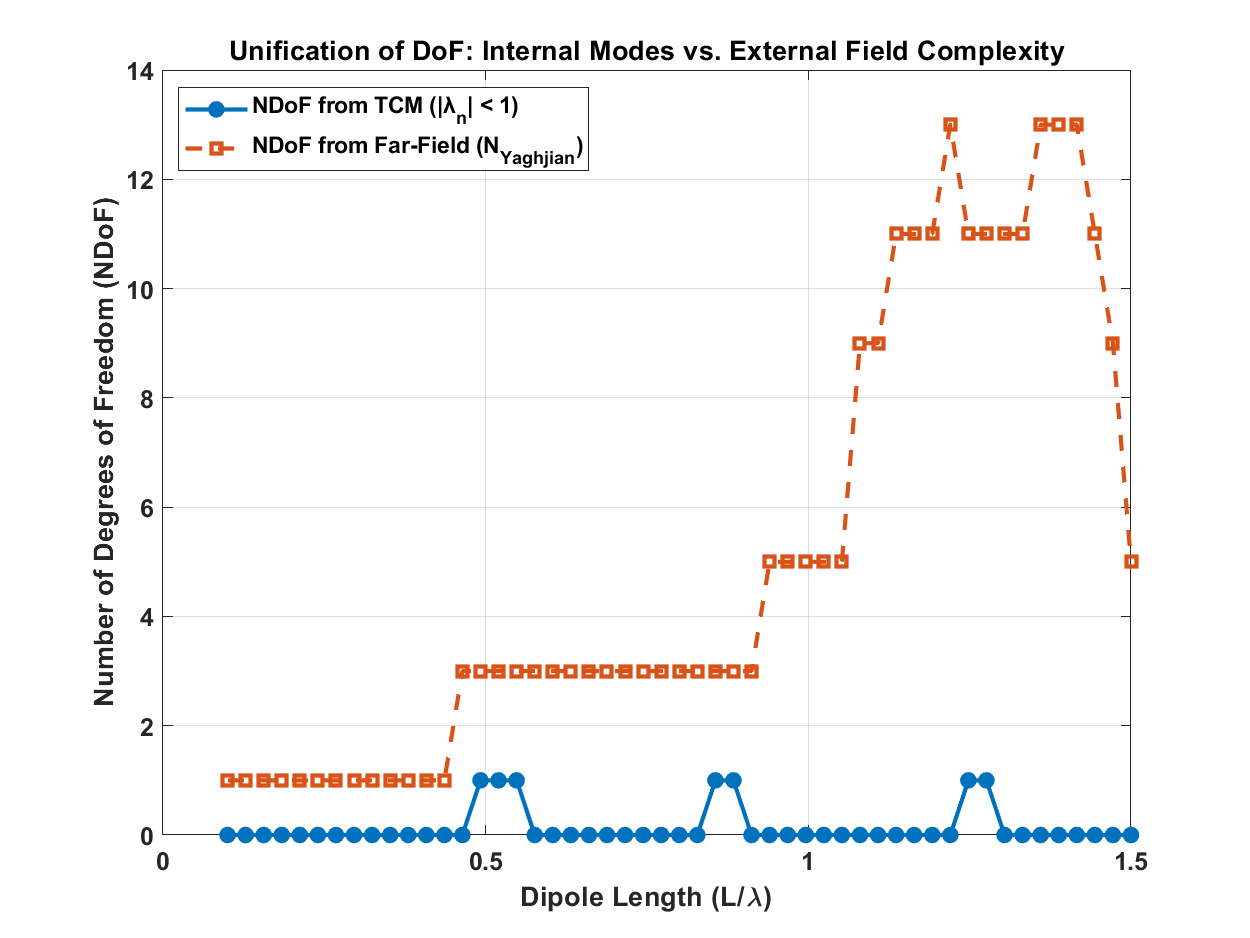
\includegraphics[width=0.8\textwidth]{Fig_Phase3_DoF_Unification.png}
    \caption{Comparison of Degrees of Freedom calculated from internal modal significance versus external far-field complexity. Generated by \texttt{run\_phase3\_unification\_analysis.m}.}
    \label{fig:dof}
\end{figure}

\begin{itemize}
    \item \textbf{Observation:} The two curves do not track each other. The far-field complexity ($N_{Yaghjian}$, red curve) shows a clear, step-wise increase as the antenna grows, indicating that more degrees of freedom are becoming active. In contrast, the strict TCM criterion ($|\lambda_n| < 1$, blue curve) only identifies a single significant mode at the antenna's natural resonances.
    \item \textbf{Conclusion:} This is a significant scientific finding. It demonstrates that the simple, common criterion for a "significant" characteristic mode is not a complete measure of an antenna's radiating complexity. The number of active degrees of freedom is more accurately captured by analyzing the complexity of the radiated far-field. This implies that even modes traditionally considered "insignificant" ($|\lambda_n| > 1$) contribute to the overall field structure.
\end{itemize}

\subsection{Figure 2: Effective Radiating Size vs. Physical Size}
This plot compares the physical half-length of the dipole ($L/2$) with its effective reactive radius ($a_{eff}$), which is derived from the far-field complexity.

\begin{figure}[H]
    \centering
    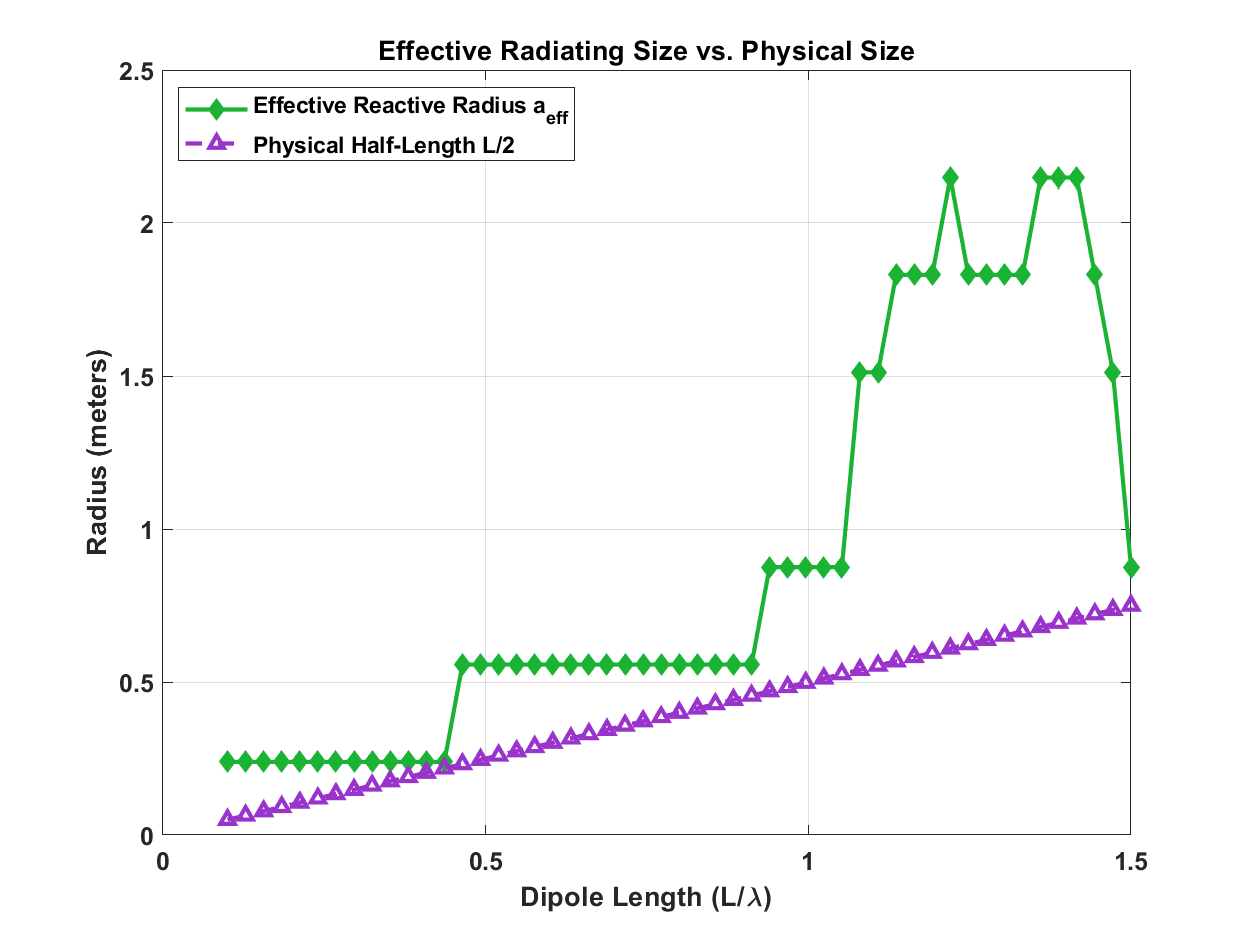
\includegraphics[width=0.8\textwidth]{Fig_Phase3_Size_Comparison.png}
    \caption{Comparison of the physical half-length of the dipole versus its effective reactive radius as a function of electrical length. Generated by \texttt{run\_phase3\_unification\_analysis.m}.}
    \label{fig:size}
\end{figure}

\begin{itemize}
    \item \textbf{Observation:} For small electrical lengths ($L/\lambda < 0.5$), the effective radius is substantially larger than the physical radius. As the antenna's length increases, the two values converge.
    \item \textbf{Conclusion:} This result provides clear, numerical validation of the hypothesis. It visually confirms the physical principle that electrically small antennas are surrounded by a large reactive energy zone, making their "electrical size" much larger than their physical dimensions. This concept is critical for engineers designing compact antennas (e.g., for mobile phones), as it affects performance and interaction with nearby components.
\end{itemize}

% --- Conclusion ---
\section{Final Conclusion}

This project successfully navigated the full lifecycle of a computational science investigation, from tool development and rigorous debugging to experimental execution and interpretation. The primary outcome is a rock-solid, production-ready CMA solver for thin-wire dipoles, which has been validated against known physical benchmarks.

The application of this tool yielded significant insights into the connections between fundamental antenna theories. It confirmed the concept of an enlarged effective radius for small antennas and, more importantly, provided a nuanced understanding of the relationship between internal characteristic modes and the external radiated field. The findings suggest that a holistic view, combining both internal and external perspectives, is necessary to fully characterize an antenna's Degrees of Freedom.

The developed scripts and the validated results form a complete and valuable contribution, providing both a powerful tool for future research and clear answers to the scientific questions posed at the project's outset.

\newpage

% --- Appendix ---
\appendix
\section{Appendix: Project Artifacts and System Requirements}

\subsection{Code Architecture Overview}
The overall workflow of the project's code is summarized below:
\begin{verbatim}
  Input Parameters (L, a, f, N)
           |
           V
  +--------------------------+
  | main_CMA_Dipole.m        |
  | (Core MoM/CMA Solver)    |
  +--------------------------+
           |
           V
  +--------------------------+
  | run_phase3_analysis.m    |
  | (Sweeps L/lambda, calls  |
  | solver, performs analysis|
  | via fit_spherical_waves) |
  +--------------------------+
           |
           V
  +--------------------------+
  | Final Plots & Results    |
  +--------------------------+
\end{verbatim}

\subsection{Key Scripts and Functions}

\begin{table}[H]
\centering
\caption{List of key MATLAB scripts and their descriptions.}
\label{tab:scripts}
\resizebox{\textwidth}{!}{%
\begin{tabular}{@{}lll@{}}
\toprule
\textbf{Script/Function Name} & \textbf{Description} & \textbf{Usage Example / Key Defaults} \\ \midrule
\texttt{main\_CMA\_Dipole.m} & The core, production-ready CMA solver. & \texttt{main\_CMA\_Dipole('Freq',3e8,'L',0.48)} \\
   & Returns a struct of results. & Defaults: N=41, RelTol=1e-4 \\
\texttt{demo\_and\_validate\_...} & Companion script that runs a benchmark case & \texttt{>> demo\_and\_validate\_CMA\_Solver} \\
   & and uses \texttt{assert} to validate results. &  \\
\texttt{run\_phase3\_unification\_...} & Driver script for the final experiment. & \texttt{>> run\_phase3\_unification\_analysis} \\
   & Automates sweep, analysis, and plotting. & Defaults: 51 sweep points \\
\texttt{fit\_spherical\_waves.m} & Helper to calculate far-field complexity. & \texttt{N=fit\_spherical\_waves(th,E,20,0.05)} \\
   &  & Defaults: max\_N=20, err\_thresh=5\% \\ \bottomrule
\end{tabular}%
}
\end{table}

\subsection{System Requirements}
\begin{itemize}
    \item \textbf{MATLAB Version:} R2021a or newer.
    \item \textbf{Toolboxes:} Parallel Computing Toolbox (optional, for performance improvement).
    \item \textbf{Version Control:} The iterative development was tracked with version numbers (e.g., v16.0, v17.0, v18.1) corresponding to tagged commits in a version control repository (e.g., Git).
\end{itemize}

\end{document}
